\documentclass{beamer}
\usetheme{Dresden}

%few useful packages ------------------------------------------------------------------
\usepackage{setspace}
\let\Tiny=\tiny %remove annoying warnings
\usepackage[english]{babel}
\usepackage[latin1]{inputenc}
\usepackage{amsmath}
\usepackage{amssymb}
\usepackage{amsthm}
\usepackage{amsfonts}
\usepackage{colortbl}
\usepackage{float}
\usepackage{xcolor}
\usepackage{eurosym}
\usepackage{chngpage}
\usepackage{fancyhdr}
\usepackage{fancyvrb}
\usepackage{float}
\usepackage{framed}
\usepackage{multirow}
\usepackage{physics}
\usepackage{graphicx}
\graphicspath{ {./images/} }
\usepackage{geometry}
\usepackage{lipsum}
\usepackage{tabularx}
\usepackage{url}

\usepackage{listings}
\lstset{frame=tblr,
	language=R,
	aboveskip=5mm,
	belowskip=5mm,
	showstringspaces=false,
	columns=flexible,
	basicstyle={\small\ttfamily},
	numbers=none,
	numberstyle=\tiny\color{gray},
	keywordstyle=\color{blue},
	commentstyle=\color{dkgreen},
	stringstyle=\color{mauve},
	breaklines=true,
	breakatwhitespace=true,
	tabsize=3
}


%---------------------------------------------------------------------------------------
\usepackage[backend=biber, style=authoryear, maxcitenames=3, citestyle=apa]{biblatex}

\addbibresource{bib.bib} 

% New Commands ----------------------------
\newcommand{\bb}{\bigbreak\noindent}

\setbeamertemplate{items}[circle]


\title{ How Do Supply Shocks to Inflation Generalise? Evidence from the Pandemic Era in Europe}
\subtitle{An NBER Working Paper}
\author{Viral V. Acharya,\\ Matteo Crosignani,\\ Tim Eisert, \& Christian Eufinger (2023)}



\begin{document}
	\begin{frame}[plain]
		\maketitle
	\end{frame}
\begin{spacing}{1.5}
	
\begin{frame}
	\tableofcontents
\end{frame}
	
\section{Introduction}
	\begin{frame}
	\frametitle{Inflation}
		\begin{center}
			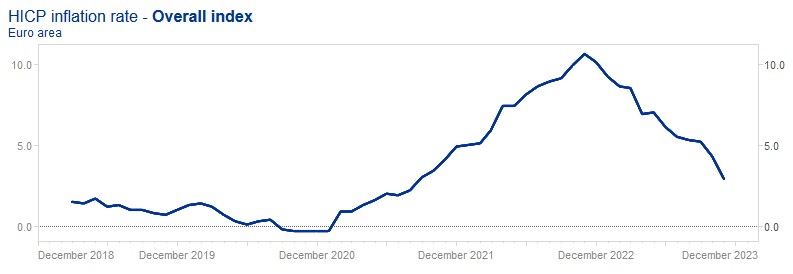
\includegraphics[width= 25em]{inflation}
		\end{center}
		\cite{blanchard2023caused}
		\begin{itemize}
			\item Sharp increases in commodity prices and sectoral shortages
		\end{itemize}
	\end{frame}
	
	\begin{frame}
		\frametitle{Frim Pricing Power \& Mark Ups}
		\begin{columns}
			\begin{column}{0.3\textwidth}
				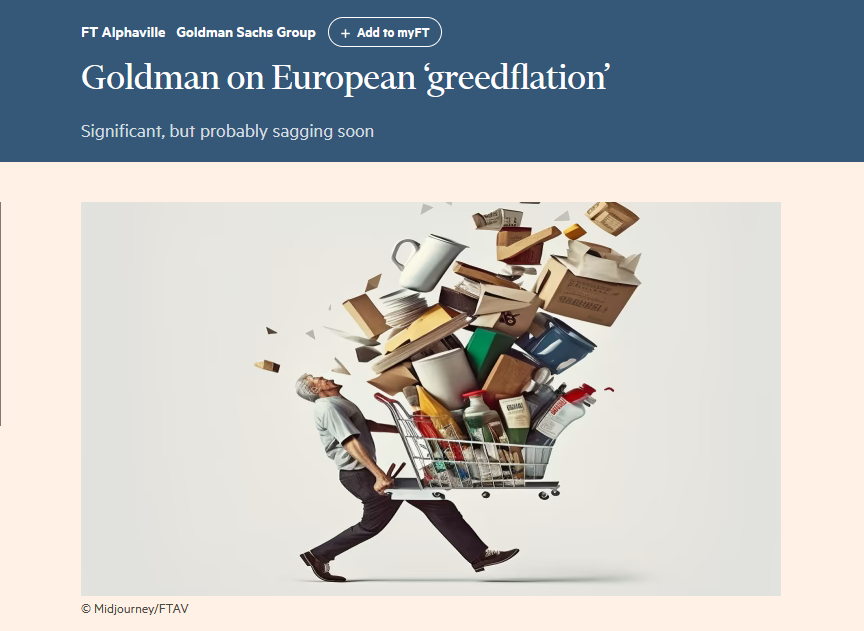
\includegraphics[width=10em]{greedflation}
			\end{column}
			
			\begin{column}{0.6\textwidth}
				\cite{franzoni2023supply}
				\begin{itemize}
					\item supply-chain constraints lead to a decrease in competition benefiting large firms
				\end{itemize}
				
				\cite{brauning2023cost}
					\begin{itemize}
						\item increased industry concentration may amplify inflationary pressures.
					\end{itemize}
				
			\end{column}
		\end{columns}
	\end{frame}
	
	\begin{frame}
		\frametitle{Inflation Expectations}
		The central contribution of this paper:
		\begin{itemize}
			\item Supply shortages lead to inflationary pressures
			\item Upward push on inflation expectations
			\item Increased inflation expectation $\rightarrow$ further increased markups
		\end{itemize}
		
		
	\end{frame}
	
	
	\begin{frame}
		\frametitle{Inflation Expectations}
		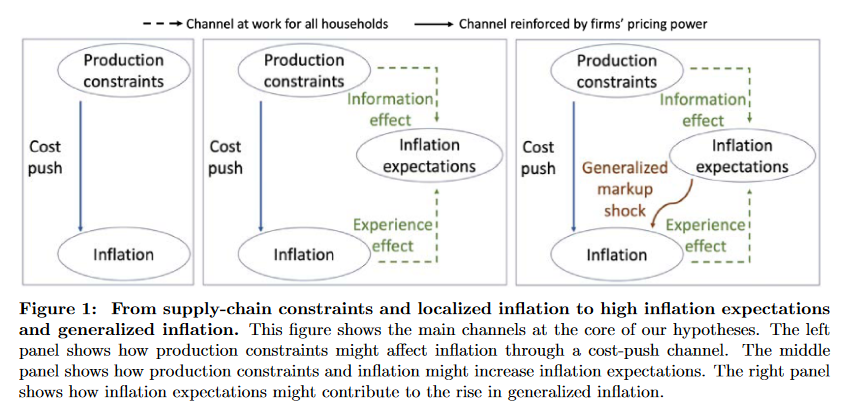
\includegraphics[width=\textwidth]{flowchart}
		
	\end{frame}



\section{Methodology}
\begin{frame}
	\frametitle{Data}
	\begin{itemize}
		\item Joint Harmonised EU Programme of Business and Consumer Surveys (BCS)
		\item ECB Consumer Expectations Survey (CES)
		\item Eurostat (PPI \& CPI)
		\item Firm-level financial data from Compustat Global
		\item Google Trends
	\end{itemize}
	
\end{frame}

\begin{frame}
	\frametitle{Regression Analysis}
	First type:\\
	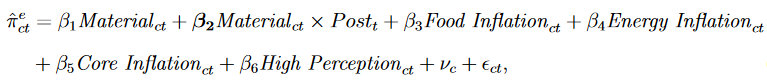
\includegraphics[width=\textwidth]{postreg}
	\bb
	Second Type:\\
	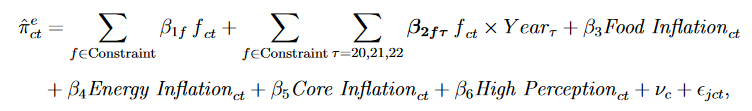
\includegraphics[width=\textwidth]{yearreg}
	
\end{frame}


\section{Findings \& Conclusion}
\begin{frame}
	\frametitle{Findings}
	
	Supply shock $\rightarrow$ inflation
	\begin{itemize}
		\item Supply Shocks associated with increases in PPI
			\begin{itemize}
				\item Firms in concentrated industries pass on higher production costs
			\end{itemize}
		\item Supply shocks associated with increases in CPI
	\end{itemize}
	\bb
	Supply shock $\rightarrow$ Inflation Expectations
	\begin{itemize}
		\item Lead to increased inflation expectations
	\end{itemize}
		
\end{frame}

\begin{frame}
	\frametitle{Findings}
	
	Supply shock $\rightarrow$ Firm Mark ups
	\begin{itemize}
		\item Firms with higher ex-ante pricing power saw increased in mark ups
	\end{itemize}
	
	Inflation Expectations $\rightarrow$ Firm Mark ups
	\begin{itemize}
		\item Some evidence to show Higher HH expectations are associated with increased mark ups in 2022
	\end{itemize}
	
\end{frame}



\begin{frame}
	\frametitle{Conclusion}
		The paper documents interactions between inflation and:
		\begin{itemize}
			\item supply-chain pressures
			\item firm pricing power
			\item and household inflation expectations
		\end{itemize}
\end{frame}

\begin{frame}
	\frametitle{Policy Implications}
	
	\begin{enumerate}
		\item Unanchored Inflation Expectations
			\begin{itemize}
				\item Decisive and clear monetary policy
				\item Transparent Communication 
			\end{itemize}
		\item Role of competitiveness
	\end{enumerate}
	
\end{frame}

\section{Extensions}
\begin{frame}
	\frametitle{Possible Issues}
	
	\begin{enumerate}
		\item Causality?
		\begin{itemize}
			\item No counterfactual. 
		\end{itemize} 
		\item Evidence of wide spread increase in mark-ups during the Pandemic is disputed \parencite{weber2022inflation}
		\begin{itemize}
			\item Inflated prices in systematically significant sectors lead to wide-spread inflationary pressures.
		\end{itemize}
		
	\end{enumerate}
	
	
\end{frame}

	


\pagebreak
\printbibliography

\end{spacing}		
\end{document}
